\documentclass[conference]{IEEEtran}
\IEEEoverridecommandlockouts
% The preceding line is only needed to identify funding in the first footnote. If that is unneeded, please comment it out.
\usepackage{cite}
\usepackage{amsmath,amssymb,amsfonts}
\usepackage{algorithmic}
\usepackage{graphicx}
\usepackage{textcomp}
\usepackage{xcolor}
\def\BibTeX{{\rm B\kern-.05em{\sc i\kern-.025em b}\kern-.08em
    T\kern-.1667em\lower.7ex\hbox{E}\kern-.125emX}}
\begin{document}

\title{PharmaSEE\\
% {\footnotesize \textsuperscript{*}Note: Sub-titles are not captured in Xplore and
% should not be used}
% \thanks{Identify applicable funding agency here. If none, delete this.}
}

\author{\IEEEauthorblockN{ Dayoung Yun}
\IEEEauthorblockA{\textit{Department of Information Systems}\\
\textit{Hanyang University}\\
Seoul, South  Korea\\
yundayoung1028@gmail.com}
\and
\IEEEauthorblockN{Morgan Jeon}
\IEEEauthorblockA{\textit{Department of Information Systems}\\
\textit{Hanyang University}\\
Seoul, South  Korea\\
momopeach9816@gmail.com}
\and
\IEEEauthorblockN{KyoungWhan Mheen}
\IEEEauthorblockA{\textit{Department of Information Systems}\\
\textit{Hanyang University}\\
Seoul, South  Korea\\
kwmheen@hanyang.ac.kr}
\and
\IEEEauthorblockN{Dohyeong Han}
\IEEEauthorblockA{\textit{Department of Information Systems}\\
\textit{Hanyang University}\\
Seoul, South  Korea\\
dohan2038@gmail.com}
\and
\IEEEauthorblockN{Miju Kang}
\IEEEauthorblockA{\textit{Department of Information Systems}\\
\textit{Hanyang University}\\
Seoul, South  Korea\\
mj0904meeju@gmail.com}
\and
\IEEEauthorblockN{}
}

\maketitle

\begin{abstract}
PharmaSEE is a service that notifies users information of medicines like usage and whether they took it or not. Target customers of our new service are visually handicapped people who have difficulties checking types and usages of medicines or people who cannot remember well whether they had medicines or not. By using the application, the user can take the photo of the pill and get its information from a NUGU speaker in voice. This function is for people who are visually impaired. Also, it recognizes how to take pills and alerts you to take pills/nutritional supplements. Users can save data to check if they took it. People who take medicines regularly can use it. With regards to data resources, we use a pill image dataset provided by the Ministry of Food And Drug Safety of Korea. There may be possible additional features. For instance, it can recommend over-the-counter medicine according to symptoms. Or we can apply this service to nutritional supplements or vitamins.
\end{abstract}

\begin{IEEEkeywords}
Image Recognition, Mobile Application, AI Speaker
\end{IEEEkeywords}

\section{Introduction}
\subsection{Motivation}
Drugs are essential factors for modern people, from treating diseases to taking vitamins to improve their health. In this light, we planned this project to eliminate obstacles that make certain people uncomfortable when taking medicine in their lives.

There are two main cases of taking medicine periodically. There are nutritional supplements taken for therapeutic purposes and vitamins taken to improve health quality. In the case of nutritional supplements, it is easy to forget to take them when you have a busy morning. In a similar context, the medication interval is also set, but it is easy to take the medication arbitrarily without properly measuring the medication interval. In this situation, we felt that a program was needed to inform people the proper time to take each particular drug.

From a different point of view, there is a class that feels very uncomfortable taking medicine. They are the visually impaired, who “can’t see” what drugs they are taking now. Most medicines are currently marked only as "drugs" in Braille, so it is not easy to know what kind of medicine they are holding and what kind of efficacy the medicines have. Therefore, in order to help them take medicine, we thought that an additional function to recognize the medicine was needed.\\

\section{Problem statement(user's needs)}
-Users often tend to forget the medicine they need to take.\\

-Users can check drug information through the app when the name of the drug is difficult or the manual is lost. Drug information includes the name, intake method, expiration date, and side effects of the drug.\\

-Users can check the interaction between taking drugs to prevent the risk of wrong intake.\\

-Users can prevent duplicate intake by leaving records of taking drugs.\\

\subsection{Research on related  software}
A. Korea Pharmaceutical Information Center
The Korean Pharmaceutical Information Center provides pill searching services on their websites. People can search the pill by its shape, color, and formulation. After selecting the shape and color, the website shows the pills that meet the conditions. The name, company and ingredient of the pill is provided in the website, but the effect of the pill is not included. Also, it does not provide a system for the people who are visually impaired.\\

B. HealthMore
HealthMore is an application for people who are visually impaired. It is provided in the  iPhone Appstore and Google Playstore. In the application, people can take the photo of the barcode of drugs and get the information. Also, the information of pills in a prescription can be informed if the prescription includes a QR code. When people take the photo of the QR code in the prescription, the list of the pills, name of the hospital and doctor, and the date medicines prescribed  can be known. The application also provides searching functions in voice or text. If a user presents his personal health information, the caution for some drugs that are not good for him is also provided.


\section{Requirement Analysis}
\subsection{Mobile Application}\label{AA}
Users can access the main services provided by PharmaSEE through a mobile application. Native applications for Android and iOS will be provided. The user can access services such as pill image recognition, personal medication list, medication intake calendar and personalized notifications. The mobile app will be connected to a cross-platform backend server that will also communicate with the NUGU device in order to provide voice assistance for users that are not used to the mobile interface. The main functions of the mobile application are as follows.\\
\paragraph{Loading UI}The users will see a loading UI while waiting for the mobile app to boot. The PharmaSEE logo and a simple animation will indicate the user to wait for the loading process to complete.\\

\paragraph{Navigation Tab}There are several menus the user has to navigate through while using the mobile application. A navigation tab will allow the user to shift between different menus. \\
\paragraph{Main Page}The main page will display the menu icons to navigate to ‘Pill Recognition’, ‘My Medication’, etc. This will be the first page users will see upon entering the mobile application.\\

\paragraph{Pill Recognition}Users can navigate to the pill recognition menu in order to identify an unknown medicine and acquire information about it. The mobile application will open the smartphone’s built-in camera and wait for the user to take an image of the pill. If the angle is not appropriate, the app will provide guidance to the user.\\

\begin{itemize}
\item Camera: The mobile phone’s built in camera will be used to take images of the pill the user wished to identify.\\

\item Image Taking Guidance: The application will guide the user to adjust the angle or environment the image is taken. The guidance will be provided in text through the application.\\
\end{itemize}


\paragraph{Pill Information Display}After the pill has been recognized and analyzed through the image recognition model, information about the pill will be queried from the database through the backend server. The queried information contains data such as the name, manufacturer(a medicine company that made the pill), proper usage and dose, effects,possible side effects, etc. The information will be displayed in text. Also, users will be able to register the identified pill to their personal medication list (My Medication). Once the medication is registered, the user can use the medication calendar to track their intake history. Also, they can set a notification alarm to remind them to take the medication.\\

\paragraph{My Medication}Another important feature of PharmaSEE is the ‘My Medication’ section. The users can register to a list the medication they need to take daily. These medications will be organized into a calendar that will allow them to track their intake history.\\

\begin{itemize}
\item Registration (Add/Remove): The user can add medicines that they will take or are taking and remove some pills that they registered before when he/she quit taking them. \\

\item List: The user can check a list of pills that they are taking now. The pills registered by users are automatically added to the list. In addition, at the end of the period of taking a pill, it may automatically disappear from the list. Also, even if the user manually removes it by using the ‘Remove’ function, it disappears from the list.\\ 

\item Calendar: There is a personalized calendar that the users can check pill information at once. They can make an appointment to visit a doctor of a hospital or clinic again around the end of their pills period.\\

\item Notification Setting: Users can set the sound or frequency of their notifications which alert the time to take medicines.\\
\end{itemize}


\paragraph{Notification} Users can set push alarms to notify them when to take a pill they have registered. Unique sound only for this application is required so that it can make the users divide notifications of this app from other apps. This function is also very useful for visually impaired users since they can ask the NUGU speaker which specific medicine they have to take when they are notified by the push alarms from the mobile application.\\



\section{Development Environment}
\subsection{Choice of software development platform}\label{AA}
\subsubsection{Which platform and why?}
We will develop a mobile application on Windows. Our service is a kind of healthcare application, so it should be ready at hand. So our service provides a mobile application for users. We will develop both iOS and Android, so we should choose a cross-platform available technology stack. React Native will be used to develop the application. By using React Native, both Android and iOS will be supported in the same codebase. It means that we can support 99.65\% of people in Korea. \\
We will use linux based ubuntu of AWS's EC2 service as server computer. Nginx will be used as a web server. As Django cannot directly communicate with web server, we will use uWSGI python package to connect Django and web server. \\
\begin{figure}\centering
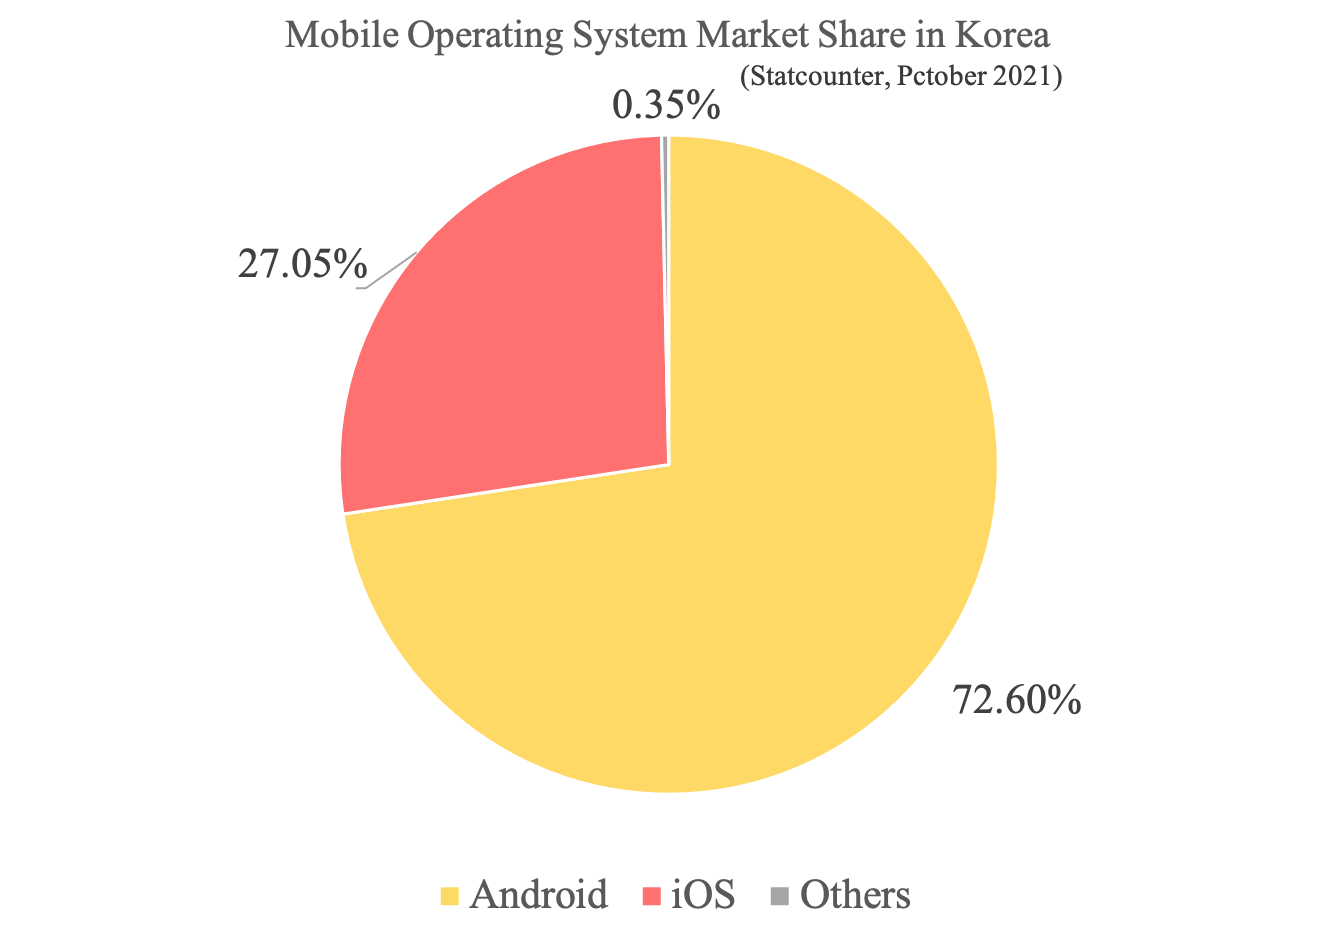
\includegraphics[width=7cm]{imagefolder/1.png}
\caption{}
\label{fig:map}
\end{figure}


\subsubsection{Which programming language and why?}
\begin{table}[htbp]
% \caption{Table Type Styles}
\begin{center}
\begin{tabular}{|p{0.1\textwidth}|p{0.25\textwidth}|}
\cline{1-2}
\textbf{Language} & \textbf{\textit{Description}} \\
\hline
Python&Python is script, dynamic type, platform independent language. 
We can check, modify, and write code immediately by the interpreter without the compilation process.
We can develop in any environment such as Windows, Linux, Mac os. 
Python has a low running curve and high scalability and portability. 
Because data learning algorithms will be implemented in a python environment, python has the advantage that it has an extensive set of libraries for artificial intelligence and machine learning. For example, Pandas library for general-purpose data analysis, Seaborn  for data visualization, and Keras, TensorFlow, Pytorch for machine learning. In addition, it is considered advantageous in that a community for problem solving is well established.\\
\hline
JSX&JSX is a JavaScript Extension Syntax used in React to easily write HTML and JavaScript together. It is usually used in React Native and also ReactJS. It is faster than normal JavaScript because it optimizes the codes while translating it to JavaScript. JSX is easy to read because it is similar to html. It is also comfortable for people who have experience in xml or JavaScript. Developers can configure the screen by components, and it increases productivity. In JSX, JavaScript expressions can be also used. \\
\hline
\end{tabular}
\label{tab1}
\end{center}
\end{table}


\subsubsection{Provide a cost estimation for your built}\\
\begin{table}[htbp]
% \caption{Table Type Styles}
\begin{center}
\begin{tabular}{|c|c|}
\cline{1-2}
\textbf{Device} & \textbf{\textit{Price(won)}} \\
\hline
Server(AWS EC2)&  \\
\hline


\end{tabular}
\label{tab1}
\end{center}
\end{table}


\subsubsection{Provide clear information about your development environment}
\begin{itemize}
  \item Pill Data Learning Model \\
It will be implemented in macOS 11.6.1 environment (Big Sur). The development will proceed in a Python virtual environment. To create a data learning model, the Python version will be downgraded to 3.7.11 for Tensorflow operation. 
  \item React Native 0.66.3
  \item Node.js 16.13.0
  \item npm 8.1.0
  \item Windows 10
  \begin{itemize}
         \item 1.80 GHz Intel i7
         \item 8GB Memory
       \end{itemize}
  \item MacOS 11.6.1(Big Sur)
  \item Visual Studio Code 1.62.1
  \item Django 3.2.9
  \item AWS EC2 instance
  \item Nginx 1.21.4
  \item Git 2.33.1
\end{itemize}

\subsection{Software in use}\label{AA}
\subsubsection{React Native}
React Native is an open source mobile application framework released by Facebook. It uses ReactJS libraries and JSX. Developers can make an application that is available for both  iOS and Android by using React Native. React Native applications can be used for both platforms simultaneously while using a single codebase. It increases productivity and makes development efficient. React Native optimizes performance by communicating with native thread through the native bridge. \\
\begin{figure}[h!]

\includegraphics[width=5cm]{imagefolder/react_native.png}
\caption{}
\label{fig:map}
\end{figure}

\subsubsection{Django}
Django is a full-stack open-source framework that can be developed both in the front-end and the back-end. Django provides ORMs that connect RDBs such as SQLite, PostgreSQL, MySQL, and Oracle with objects without using SQL queries.  Django has an active community where we can obtain information when a problem occurs. Django provides an administrator page to easily generate and change data. \\

\begin{figure}[h!]
\centering

\includegraphics[width=5cm]{imagefolder/django.png}
\caption{}
\label{fig:map}
\end{figure}

\subsubsection{TensorFlow}
TensorFlow, created in 2015 by Google Brain Team, is an open source software library for data flow programming for various tasks. It is a symbolic math library and is also used in machine learning applications such as artificial neural networks and deep learning. \\
Also It has compatibility with Keras, which is an open source neural network library. Keras provides pipelining, estimators, and eager execution which are system-specific functionality to TenseFlow. Keras functional API supports a variety of topologies with different combinations of I/O, and layers. \\
\begin{figure}[h!]
\centering

\includegraphics[width=5cm]{imagefolder/tensor.png}
\caption{}
\label{fig:map}
\end{figure}

\subsubsection{Git, Github}
Git is a tool that can manage project versions. We can copy the project to our local environment and merge it again after working. Git provides an environment where multiple people can work as a single project. Providing such an environment can speed up development and manage work details in parallel. And it can increase the stability of the project. Remote storage is required to push files committed with Git. At this time, Github is used as a remote storage. And we can also use Github as a private repository.\\

\subsection{Task Distribution}\label{AA}
\begin{table}[h!]
\begin{center}
\begin{tabular}{|p{0.1\textwidth}|p{0.25\textwidth}|}
\cline{1-2} 
\textbf{Name} & \textbf{\textit{Task Distribution}} \\
\hline
Dayoung Yun&Build the server - Mainly focus on building a pipeline for the pill image recognition service.\\
\hline
Dohyeong Han&Build the server, design API, manage DB. Manage the whole backend part.\\
\hline
Miju Kang&Connect the server and the mobile application. Configure the operation of the mobile application with the data received from the server.\\
\hline
Morgan Jeon&Let the received data be adjusted, construct the User Interface and design it by using CSS.\\
\hline
KyoungWhan Mheen&Based on the collected pill data, a code is created to analyze what the pill is taken in the picture, and send the result value to the server.\\
\hline
\end{tabular}
\label{tab1}
\end{center}
\end{table}


\section{SPECIFICATIONS}\\

\subsection{LOADING UI}Loading UI contains our application’s logo and team name, M&T. \\
\begin{figure}[h!]
\centering
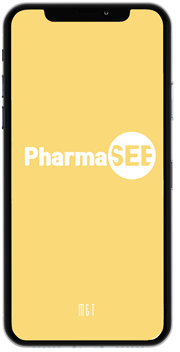
\includegraphics[width=5cm]{imagefolder/loadingui.png}
\caption{}
\label{fig:map}
\end{figure}

\subsection{MAIN PAGE}Main Page has two buttons(Pill Recognition, My Medication). If the user presses each button, it goes to the corresponding page.\\ 

\begin{figure}[h!]
\centering
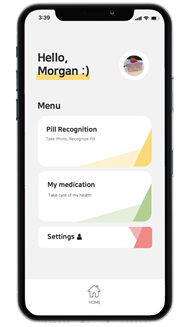
\includegraphics[width=5cm]{imagefolder/mainpage.png}
\caption{}
\label{fig:map}
\end{figure}

\subsection{PILL RECOGNITION}\\

\begin{figure}[h!]
\centering
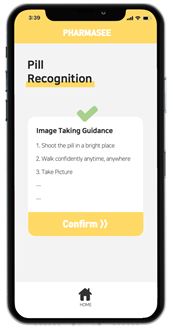
\includegraphics[width=5cm]{imagefolder/pillrecog1.png}
\caption{}
\label{fig:map}
\end{figure}

\subsubsection{Image taking guidance}The application will guide how to take an image of a pill by text. Users can take an image of the pill according to the guide.\\

\begin{figure}[h!]
\centering
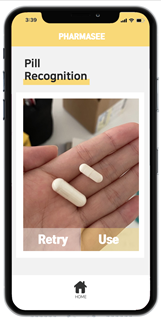
\includegraphics[width=5cm]{imagefolder/pillrecog2.png}
\caption{}
\label{fig:map}
\end{figure}

\subsubsection{Image taking page}The smartphone's built-in camera will be used to take an image of a pill. If the user wants to go back to the previous page, the user can press the previous button at the upper left.\\

\subsection{INFORMATION DISPLAY}\\

\begin{figure}[h!]
\centering
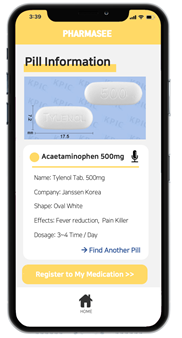
\includegraphics[width=5cm]{imagefolder/infodisplay.png}
\caption{}
\label{fig:map}
\end{figure}

\subsubsection{}After taking the photo of the pill, the image goes to the server and the server recognizes the pill. Users can see the name, company, effects and dosage of the pill in text.\\ 

\subsubsection{}It is possible to hear the information in voice through the NUGU speaker if the user touches the microphone button, or asks NUGU directly. The voice command for this is  ‘Aria, tell me the information about this pill’.\\

\subsubsection{}Users can also register the recognized pill to ‘My Medication’(a list of pills users are currently taking or have taken previously). If they want, they can identify a different pill by clicking the ‘Find Another Pill’ button.\\


\subsection{MY MEDICATION - REGISTRATION}\\


\subsubsection{}Users can register the pills they have identified through the ‘Pill Recognition’ menu. Or they can manually insert the pill’s name and intake information instead.\\

\subsubsection{}Registered pills will be uploaded to the medication list and the user will be able to add intake information to the calendar, set notifications, etc.\\

\subsection{MY MEDICATION - LIST}\\
\begin{figure}[h!]
\centering
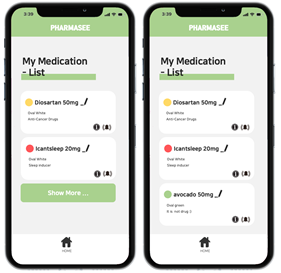
\includegraphics[width=5cm]{imagefolder/medi_list.png}
\caption{}
\label{fig:map}
\end{figure}

\subsubsection{}The users can check the list of pills they are taking.\\

\subsubsection{}The pills each have a specific color. Users can change it to other colors whatever they want.\\

\subsubsection{}It is possible to change pills’ names to nicknames instead of difficult original pill names. Users can edit it with a pencil-shaped icon located next to a pill name.\\

\subsubsection{} If users click the sign board-shaped first icon in the lower right corner inside each pill box, they can see detailed information about the pill.\\


\subsubsection{}If users click the bell-shaped second icon, they can set the notification for each pill.\\

\subsubsection{}When users click the ellipse-shaped  ‘See More’ box at the bottom, other drugs in the list appear additionally, and they can swipe to see them.\\



\subsection{MY MEDICATION - CALENDAR}\\
\begin{figure}[h!]
\centering
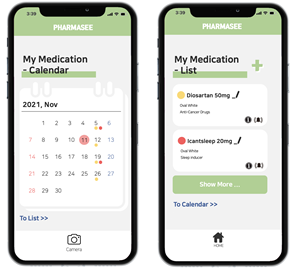
\includegraphics[width=5cm]{imagefolder/medi_calendar.png}
\caption{}
\label{fig:map}
\end{figure}

\subsubsection{}The users can check their medication schedule intuitively by looking at the calendar.\\

\subsubsection{}The calendar has a sign that denotes today as a pink circle. Also, small circles of which each color is designated color for the pills he/she is taking are marked under the date. \\

\subsubsection{}Users can swipe to the previous or next month.\\

\subsection{MY MEDICATION - NOTIFICATION}\\
\begin{figure}[h!]
\centering
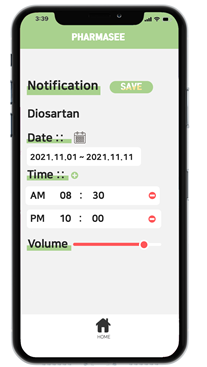
\includegraphics[width=5cm]{imagefolder/noti.png}
\caption{}
\label{fig:map}
\end{figure}

\subsubsection{}In the ‘List’ menu, each medication card contains a bell-shaped icon in the lower right corner. Users can click on this icon to open the ‘Notification Settings’ page.\\

\subsubsection{}In this page users can customize the notification setting of the pill they chose.\\

\subsubsection{}Date - Clicking on the calendar button next to the ‘Date’ section will open a calendar pop up. Users can select the starting and termination date of their medication period. \\

\subsubsection{}Time - Users will also select the time they want to be notified. If they have to take the medication more than once daily, they can add several timings by clicking on the + icon. \\

\subsubsection{}Sound - Users can enable or disable sound notifications by toggling the button in the ‘Sound’ section. If they choose not to use any sound, they will only receive a push message from the mobile application with a vibration notification. \\

\subsubsection{}Save - Once users are satisfied with all the settings, they can click on the ‘Save’ button in order to resume to the medication list page.\\



\subsection{NUGU INTERFACE}Users can use the NUGU speaker with our mobile application. They can let NUGU do some actions by giving them instructions in voice. Users’ instructions will be converted to a string by the backend proxy server through NUGU SDK. These strings will be sent to the API server which will interpret them as commands and perform appropriate actions.\\





\begin{itemize}%[leftmargin=1em]
  \renewcommand{\labelitemi}{$\rightarrow$}
 \item User’s Voice Command \\
 
 \item Intent Extracted by NUGU\\
 
 \item Action & Parameters Sent to Backend Proxy\\
 
 \item REST API Response Processed by Backend Proxy\\
 
 \item Respond in Voice Through NUGU + Perform Appropriate Actions in Mobile Application\\
\end{itemize}


\section*{Role Assignment}
\begin{table}
% \caption{Table Type Styles}
\begin{center}
\begin{tabular}{|p{0.1\textwidth}|p{0.06\textwidth}|p{0.25\textwidth}|}
\cline{1-3} 
\textbf{Role} & \textbf{\textit{Name}}& \textbf{\textit{Task Description}}\\
\hline
User/Customer&All&The person who plays the role of User/Customer collects information from users necessary for application development through a survey. He determines the main customer of the application. He prepares surveys and interviews. He analyzes the results of surveys and interviews. Based on the analysis of results, the functions and complementary points necessary for application development are shared. \\
\hline
Backend Developer&Dayoung Yun, Dohyeong Han&Backend developers think about backend systems which are needed in developing projects like using databases with SQL queries. We manage the server-side and database related to the process of a website, web application or mobile solution. As a backend developer, as many languages are provided like python, Java, Node.js, JavaScript.\\
\hline
Frontend Developer&Miju Kang,
Morgan Jeon&A frontend developer makes the environments for the users. In this project, the frontend developer also designs the UI/UX for the application. She considers user convenience and implementing design on websites and applications. It is important to hide the bug in the front, so that the user cannot notice the problem. As a frontend developer, the ability to use html, javascript and css is needed.\\
\hline
AI Developer&Kyoung Whan Mheen&The AI developer will make the pipeline that processes images and applies machine learning algorithms to classify the images taken by the user. The AI developer needs to make sure the machine learning model is making plausible predictions and is also responsible for the deployment of the pipeline.\\
\hline
Development Manager&Morgan Jeon&Development manager has to control the whole process of  software development. Therefore, it’s important to communicate with all team members for a development manager. Also,a development manager should read the situation of a market, think up essential services and suggest it to other team members. Finally, the development manager has to listen to and summarize the voice of customers and notify it to developers for service updates.\\
\hline

\end{tabular}
\label{tab1}
\end{center}
\end{table}

\begin{figure}[h!]
\caption{Role assignments of team members.}
\label{fig}
\end{figure}




















\end{document}
